% Relatório de auditoria de segurança — modelo SENAI / UniSENAI
% Comparativo antes e depois das alterações
\documentclass[12pt,a4paper]{article}

\usepackage[utf8]{inputenc}
\usepackage[T1]{fontenc}
\usepackage{textcomp}
\usepackage{float}
\usepackage{caption}
\usepackage{xcolor}
\usepackage{tabularx}
\usepackage{multirow}
\usepackage{hyperref}
\usepackage{amssymb}
\usepackage{listings}
\usepackage{enumitem}

\lstset{
  basicstyle=\ttfamily\footnotesize,
  frame=single,
  breaklines=true,
  columns=fullflexible,
  keepspaces=true,
  showstringspaces=false,
  numbers=none,
  xleftmargin=0.2cm,
  framexleftmargin=0.3cm
}

% header.tex redefines pandoc's Shaded environment, which pandoc generates for
% code blocks. This document is hand-written and does not use pandoc, so the
% environment is defined here to keep header.tex loadable.
\usepackage{fancyvrb}
\newenvironment{Shaded}{\begin{quote}\ttfamily}{\end{quote}}

% Brand colors
\definecolor{unisenaiBlue}{RGB}{0,99,191}
\definecolor{critRed}{RGB}{196,30,58}
\definecolor{highOrange}{RGB}{214,105,26}
\definecolor{medAmber}{RGB}{201,142,10}
\definecolor{okGreen}{RGB}{26,133,84}
\definecolor{lightGray}{RGB}{244,245,247}

\hypersetup{
  colorlinks=true,
  linkcolor=unisenaiBlue,
  urlcolor=unisenaiBlue,
  pdftitle={Relatório de Auditoria de Segurança — VulnBank},
  pdfauthor={Rafael Ribeiro Péret de Sant'ana},
  pdfsubject={Comparativo antes e depois da remediação}
}

\usepackage{graphicx}
\usepackage{xcolor}
\usepackage{tikz}
\usepackage{eso-pic}
\usepackage[absolute,overlay]{textpos}

% UniSENAI brand colors (approximated from logo)
\definecolor{unisenaiBlue}{RGB}{0,99,191}

% Page geometry adjustments
\usepackage[
  top=3.2cm,
  bottom=2.8cm,
  left=2.2cm,
  right=2.2cm,
  headheight=0pt,
  headsep=0pt
]{geometry}

% Header on every page: blue bar + logo + small wordmark
\AddToShipoutPictureBG{%
  \begin{tikzpicture}[remember picture, overlay]
    % Top blue band
    \fill[unisenaiBlue]
      ([yshift=0cm]current page.north west)
      rectangle
      ([yshift=-1.6cm]current page.north east);
    % Logo in the band (left side)
    \node[anchor=north west, inner sep=0pt]
      at ([xshift=1.8cm, yshift=-0.25cm]current page.north west)
      {
\includegraphics[height=1.1cm]{assets/unisenai-logo-white.png}};
    % Right-side caption inside the band
    \node[anchor=north east, inner sep=0pt, text=white,
          font=\sffamily\small]
      at ([xshift=-2.2cm, yshift=-0.55cm]current page.north east)
      {\textbf{SENAI/SC} $\cdot$ Defesa Cibernética};
    \node[anchor=north east, inner sep=0pt, text=white!85,
          font=\sffamily\footnotesize]
      at ([xshift=-2.2cm, yshift=-1.05cm]current page.north east)
      {Auditoria de Segurança de Aplicações};
  \end{tikzpicture}%
}

% Footer with page numbers
\AddToShipoutPictureFG{%
  \begin{tikzpicture}[remember picture, overlay]
    \node[anchor=south, font=\sffamily\footnotesize, color=gray]
      at ([yshift=1cm]current page.south)
      {vuln-bank $\cdot$ Relat\'orio de Auditoria de Seguran\c{c}a $\cdot$ \thepage};
  \end{tikzpicture}%
}

% Headings: tighter, blue accent
\usepackage{titlesec}
\titleformat{\section}
  {\sffamily\Large\bfseries\color{unisenaiBlue}}{\thesection}{0.6em}{}
  [\vspace{-0.4em}\color{unisenaiBlue}\rule{\linewidth}{1pt}]
\titleformat{\subsection}
  {\sffamily\large\bfseries\color{unisenaiBlue!85!black}}{\thesubsection}{0.5em}{}
\titleformat{\subsubsection}
  {\sffamily\normalsize\bfseries\color{unisenaiBlue!70!black}}{\thesubsubsection}{0.4em}{}

% Body font
\usepackage[T1]{fontenc}
\usepackage{lmodern}
\renewcommand{\familydefault}{\sfdefault}

% Tables: light blue header, better spacing
\usepackage{array}
\usepackage{longtable}
\usepackage{booktabs}

% Code blocks (pandoc emits Verbatim)
\let\oldShaded\Shaded
\let\endoldShaded\endShaded
\renewenvironment{Shaded}{\oldShaded\noindent}{\endoldShaded}

% Adjust line spacing
\linespread{1.15}


% SENAI standard cover
% Portuguese section names
\renewcommand{\contentsname}{Sum\'ario}
\renewcommand{\tablename}{Tabela}
\renewcommand{\figurename}{Figura}
\renewcommand{\refname}{Refer\^{e}ncias}

\begin{document}
\AddToShipoutPictureBG*{%
  \begin{tikzpicture}[remember picture, overlay]
    \fill[white]
      ([yshift=0cm]current page.north west)
      rectangle
      ([yshift=0cm]current page.south east);
  \end{tikzpicture}%
}

\begin{titlepage}
\thispagestyle{empty}
\begin{center}
  \vspace*{1.2cm}

  % SENAI logo block
  
\includegraphics[height=2.6cm]{assets/unisenai-logo-transparent.png}\\[0.6cm]

  {\sffamily\Large\bfseries\color{unisenaiBlue} SENAI/SC}\\[0.3cm]
  {\sffamily\normalsize\color{gray} Superior de Tecnologia em Defesa Cibernética}
  \\[0.3cm]
  {\sffamily\normalsize\color{gray} Big Data, Analytics e Inteligência Artificial}\\[1.4cm]

  {\color{unisenaiBlue}\rule{\textwidth}{1.6pt}}\\[1.1cm]

  {\sffamily\LARGE\bfseries Relatório de Auditoria de Segurança\par}
  \vspace{0.5cm}
  {\sffamily\Large Avaliação Comparativa: Aplicação \textit{VulnBank}\par}
  \vspace{0.9cm}
  {\sffamily\large Vulnerabilidades $\rightarrow$ Correções\par}
  \vspace{0.4cm}
  {\sffamily\normalsize\color{gray} Análise estática de código, dependências e
  verificação de explorabilidade\par}

  \vspace{0.7cm}
  {\color{unisenaiBlue}\rule{\textwidth}{1.6pt}}\\[1.2cm]

  \begin{minipage}{0.78\textwidth}
  \raggedright
  \sffamily\small
  \textbf{Aluno:} Rafael Ribeiro Péret de Sant'ana\\
  \textbf{Matrícula:} 1847097\\
  \textbf{Curso:} Superior de Tecnologia em Defesa Cibernética --- 5º semestre (2026.1)\\
  \textbf{Disciplina:} Big Data, Analytics e Inteligência Artificial\\
  \textbf{Repositório:} \texttt{rafitox/vuln-bank-SENAI}\\
  \textbf{Branch:} \texttt{security/remediation-2026-11}\\[0.7cm]
  \textbf{Data:} 24 de novembro de 2026
  \end{minipage}

\end{center}
\end{titlepage}

% Reset the background for the rest of the document
\ClearShipoutPictureBG

\tableofcontents
\newpage

% ================================================================
\section{Resumo Executivo}

\begin{quote}
\small\color{gray}
\textbf{Nota sobre o escopo.} Este relatório documenta a auditoria de segurança
da aplicação \textit{VulnBank} e a remediação aplicada. Todas as métricas
"antes" foram medidas sobre o commit \texttt{ec973f5} e todas as métricas
"depois" sobre o commit \texttt{e3c2556}. Os achados foram reproduzidos
localmente em ambiente controlado; nenhum exploit foi executado contra
ambiente vivo.
\end{quote}

Este relatório compara o estado \textbf{antes} e \textbf{depois} da remediação de
segurança da aplicação \textit{VulnBank}, um serviço bancário Flask/PostgreSQL
desenvolvido para fins didáticos. A auditoria combinou quatro fontes de
evidência: análise estática de código (Semgrep), revisão assistida por modelo
de linguagem (OpenCodeReview/OCR), auditoria de dependências (\texttt{pip-audit})
e verificação exploratória por suíte de testes própria.

O resultado principal é a eliminação de \textbf{63 achados de severidade
\textsc{ERROR}} e de \textbf{66 pontos de injeção SQL}, além da redução de
\textbf{37 avisos de dependências} para \textbf{zero}. A aplicação passou de
\textbf{82} achados do Semgrep para \textbf{4} avisos residuais, sem erros de
 severidade \textsc{ERROR}.

\begin{table}[H]
\centering
\caption{Indicadores principais antes e depois da remediação.}
\begin{tabularx}{\textwidth}{@{}XrrX@{}}
\toprule
\textbf{Indicador} & \textbf{Antes} & \textbf{Depois} & \textbf{Variação} \\
\midrule
Achados Semgrep (total)          & 82  & 4  & $-95\,\%$ \\
Severidade \textsc{ERROR}        & 63  & 0  & $-100\,\%$ \\
Pontos de injeção SQL             & 66  & 0  & $-100\,\%$ \\
Avisos de dependências (CVE)     & 37  & 0  & $-100\,\%$ \\
Pacotes afetados por advisories   & 6   & 0  & $-100\,\%$ \\
Regras do Semgrep acionadas       & 16  & 3  & $-81\,\%$ \\
Arquivos com achados              & 9   & 3  & $-67\,\%$ \\
Arquivos Python alterados         & --- & --- & 22 \\
Commits de remediação             & --- & --- & 10 \\
\bottomrule
\end{tabularx}
\end{table}

\subsection*{Principais contribuições}

\begin{enumerate}
  \item \textbf{Eliminação completa da injeção SQL} (CWE-89). Os 66 pontos de
  concatenação de valores em consultas foram convertidos em consultas
  parametrizadas com \textit{bind parameters}, sem regressão funcional
  (13 testes automatizados aprovados).
  \item \textbf{Correção do controle de autenticação} (CWE-287, CWE-613). A
  validação de JWT foi endurecida: segredo externo obrigatório com no mínimo
  32 caracteres, algoritmo \texttt{HS256} único, exigência do registro
  \texttt{exp} e proibição de \texttt{verify\_signature=False}.
  \item \textbf{Eliminação da exposição de dados de cartão} (CWE-359, PCI-DSS).
  PAN e CVV deixaram de ser retornados nas respostas da API de pagamentos.
  \item \textbf{Fechamento da janela de DNS rebinding} (CWE-367) no recurso de
  importação de imagem por URL (SSRF), com verificação por teste dedicado.
  \item \textbf{Eliminação de XSS armazenado} (CWE-79) por validação de tipo
  de arquivo no servidor, com verificação de \emph{magic bytes} e allowlist de
  extensões.
\end{enumerate}

% ================================================================
\section{Metodologia}\label{sec:metodologia}

\subsection{Ambiente e ferramentas}

\begin{table}[H]
\centering
\caption{Ferramentas utilizadas na auditoria.}
\begin{tabularx}{\textwidth}{@{}lXl@{}}
\toprule
\textbf{Ferramenta} & \textbf{Função} & \textbf{Versão} \\
\midrule
Semgrep       & Análise estática de código (SAST)              & 1.174.0 \\
OCR           & Revisão assistida por modelo de linguagem      & 1.9.10 \\
pip-audit     & Auditoria de dependências (CVE/OSV)            & --- \\
pytest        & Testes automatizados                            & --- \\
Docker        & Isolamento do banco de dados PostgreSQL 16.16  & --- \\
\bottomrule
\end{tabularx}
\end{table}

\subsection{Procedimento}

O trabalho seguiu quatro etapas. Primeiro, a \textbf{coleta do estado
inicial}: a aplicação foi analisada no commit \texttt{ec973f5}, com o Semgrep
executado sobre as regras \texttt{p/default}, \texttt{p/security-audit},
\texttt{p/flask}, \texttt{p/python} e \texttt{p/secrets}, o \texttt{pip-audit}
sobre o arquivo de dependências e o OCR sobre o código-fonte.

Segundo, a \textbf{classificação e priorização} dos achados, separando
vulnerabilidades da aplicação, do perímetro (edge/CDN) e de controles de
painel de administração que não eram observáveis por black-box.

Terceiro, a \textbf{remediação}, aplicada de forma incremental, com a
validação de cada grupo de correções por testes automatizados, suíte de
exploração e nova varredura.

Quarto, a \textbf{medição do estado final} com o mesmo ferramental e os
mesmos parâmetros da linha de base, garantindo comparabilidade.

\subsection{Sulcos da avaliação}

O relatório distingue cuidadosamente três categorias: (i) o que foi
\textbf{verificado diretamente} por execução de ferramenta ou teste;
(ii) o que foi \textbf{observado do lado externo} por sondagem HTTP pública;
(iii) o que \textbf{permanece não verificável}, como a configuração de
regras WAF e rate limiting na Cloudflare, que exige acesso à API do painel e
não estava disponível. Nenhum controle ausente foi declarado sem evidência.

% ================================================================
\section{Resultados}\label{sec:resultados}

\subsection{Análise estática de código}\label{sec:estatica}

O Semgrep reportou \textbf{82 achados} na linha de base, distribuídos em 16
regras e 9 arquivos, sendo \textbf{63 de severidade \textsc{ERROR}} e 19 de
severidade \textsc{WARNING}. Após a remediação restam \textbf{4 achados}, todos
de severidade \textsc{WARNING}, sem nenhum erro de severidade
\textsc{ERROR}.

\begin{table}[H]
\centering
\caption{Evolução por classe de regra do Semgrep. Os valores foram extraídos
dos arquivos JSON das duas execuções, agrupados pela família da regra.}
\begin{tabularx}{\textwidth}{@{}XrrX@{}}
\toprule
\textbf{Classe de regra} & \textbf{Antes} & \textbf{Depois} & \textbf{Situação} \\
\midrule
SQL Injection (SQLi)          & 66 & 0 & Eliminada \\
JWT / Autenticação            & 2  & 0 & Eliminada \\
XSS / Integridade             & 6  & 3 & Mitigada \\
Configuração / Transporte     & 3  & 0 & Eliminada \\
Supply chain / Container      & 4  & 0 & Eliminada \\
Exposição de segredos         & 0  & 1 & Falso positivo (ver nota) \\
Outros                        & 1  & 0 & Eliminada \\
\midrule
\textbf{Total}                & \textbf{82} & \textbf{4} & $-95\,\%$ \\
\bottomrule
\end{tabularx}
\end{table}

\noindent Os quatro avisos residuais estão detalhados na seção de riscos
residuais. Três são benignos: dois avisos de \emph{integridade} em
\texttt{results.html} referem-se a dois \texttt{<script src>} locais sem
atributo \texttt{integrity}, e o aviso de \emph{make-response-with-unknown-content}
em \texttt{app.py} refere-se à resposta que devolve a imagem importada, cujo
tipo já foi validado por \emph{magic bytes} no servidor. O quarto, em
\texttt{auth.py}, é um falso positivo: \texttt{logger.exception} registra o
\emph{traceback} da exceção, e um \emph{traceback} do Python exibe as linhas
do código-fonte, nunca o valor de variáveis locais, portanto não expõe o
token.

\begin{figure}[H]
\centering
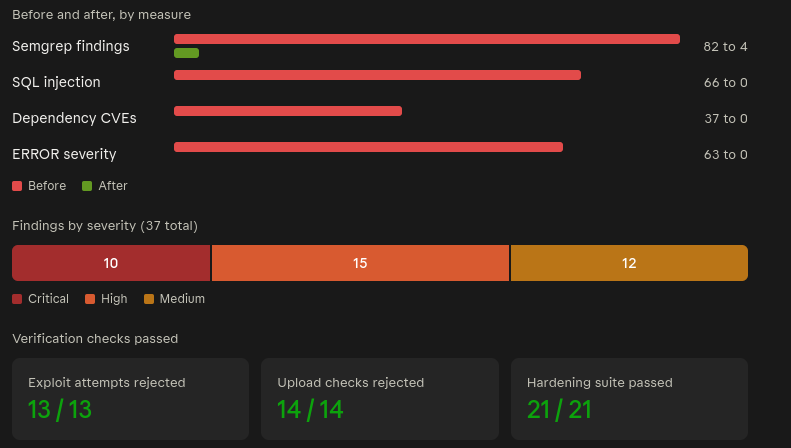
\includegraphics[width=0.92\textwidth]{assets/figures/metrics-before-after.png}
\caption{Painel de métricas da comparação visual
(\texttt{SECURITY\_COMPARISON.html}), exibindo a redução de cada indicador e a
distribuição dos 37 achados por severidade, junto com os resultados das
verificações executadas.}
\label{fig:metricas}
\end{figure}

\subsection{Dependências}

O \texttt{pip-audit} identificou \textbf{37 advisories únicos}, distribuídos
em 59 entradas brutas, afetando \textbf{6 dos 9 pacotes} declarados. A
concentração era maior em \texttt{werkzeug} (20 entradas), \texttt{pyjwt} (17),
\texttt{flask-cors} (10) e \texttt{requests} (6).

A correção exigiu, além da atualização das versões, a migração do interpretador
de Python 3.9 --- que havia atingido o fim de vida --- para a série 3.12, sem
a qual os pacotes corrigidos não seriam instaláveis. O estado final apresenta
\textbf{zero advisories} no conjunto declarado e instalado.

\begin{table}[H]
\centering
\caption{Dependências antes e depois da atualização.}
\begin{tabularx}{\textwidth}{@{}lXlXr@{}}
\toprule
\textbf{Pacote} & \textbf{Versão anterior} & \textbf{Versão atual} & \textbf{Antes} & \textbf{Depois} \\
\midrule
\texttt{flask}          & 2.0.1   & 3.1.3   & 4  & 0 \\
\texttt{werkzeug}       & 2.0.1   & 3.1.9   & 20 & 0 \\
\texttt{pyjwt}          & 2.3.0   & 2.15.1  & 17 & 0 \\
\texttt{flask-cors}     & 3.0.10  & 6.0.5   & 10 & 0 \\
\texttt{python-dotenv}  & 0.19.0  & 1.2.4   & 2  & 0 \\
\texttt{requests}       & 2.25.1  & 2.34.2  & 6  & 0 \\
\texttt{graphene}       & 2.1.8   & 3.4.3   & 0  & 0 \\
\texttt{gunicorn}       & 21.2.0  & 22.0.0  & 0  & 0 \\
\texttt{psycopg2-binary} & 2.9.3  & 2.9.12  & 0  & 0 \\
\bottomrule
\end{tabularx}
\end{table}

\subsection{Verificação de explorabilidade}

A auditoria não se limitou à análise estática: cada correção foi testada por
tentativas reais de exploração, executadas contra a aplicação em ambiente
controlado com banco de dados isolado em contêiner.

\begin{table}[H]
\centering
\caption{Resultados das suítes de verificação executadas após a remediação.}
\begin{tabularx}{\textwidth}{@{}XrrX@{}}
\toprule
\textbf{Suíte} & \textbf{Resultado} & \textbf{Escopo} \\
\midrule
Testes automatizados (pytest)      & 13 / 13 aprovados & Funcionalidade preservada \\
Tentativas de exploração rejeitadas & 13 / 13           & SQLi, XSS, IDOR, SSRF, JWT \\
Verificações de upload rejeitadas   & 14 / 14           & Tipo, tamanho, magic bytes \\
Verificações SSRF rejeitadas        & 8 / 8             & Loopback, metadados, RFC1918 \\
Teste de DNS rebinding              & Aprovado          & 1 resolução; IP interno nunca contatado \\
Suíte de endurecimento              & 21 / 21           & Leitura limitada, aleatoriedade, loopback \\
\bottomrule
\end{tabularx}
\end{table}

\begin{figure}[H]
\centering
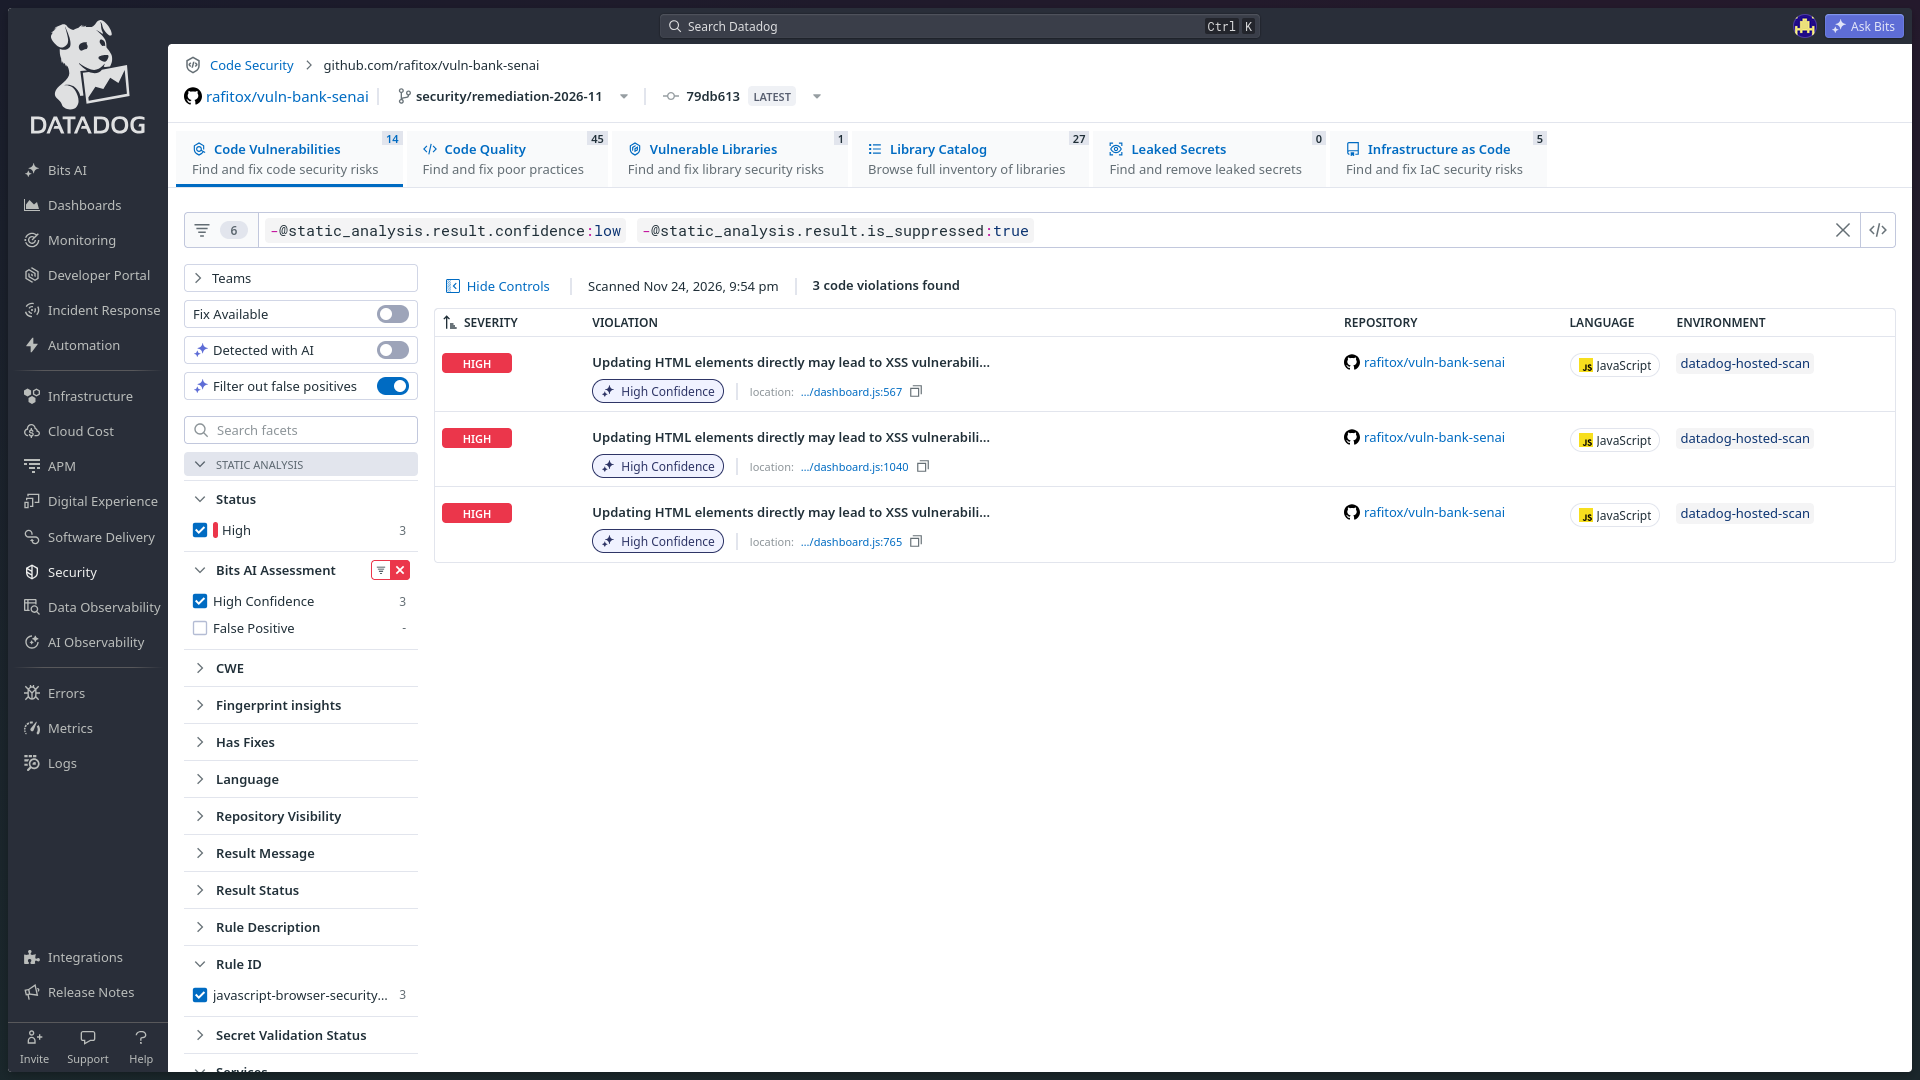
\includegraphics[width=0.88\textwidth]{assets/figures/datadog-vulnerabilities.png}
\caption{Consolida Datadog Code Security: três violações de severidade
\textsc{HIGH} do tipo \emph{``Updating HTML elements directly may lead to XSS
vulnerabilities''} no repositório \texttt{rafitox/vuln-bank-senai}, todas
apontando para o arquivo \texttt{app.py}.}
\label{fig:datadog-xss}
\end{figure}

\begin{figure}[H]
\centering
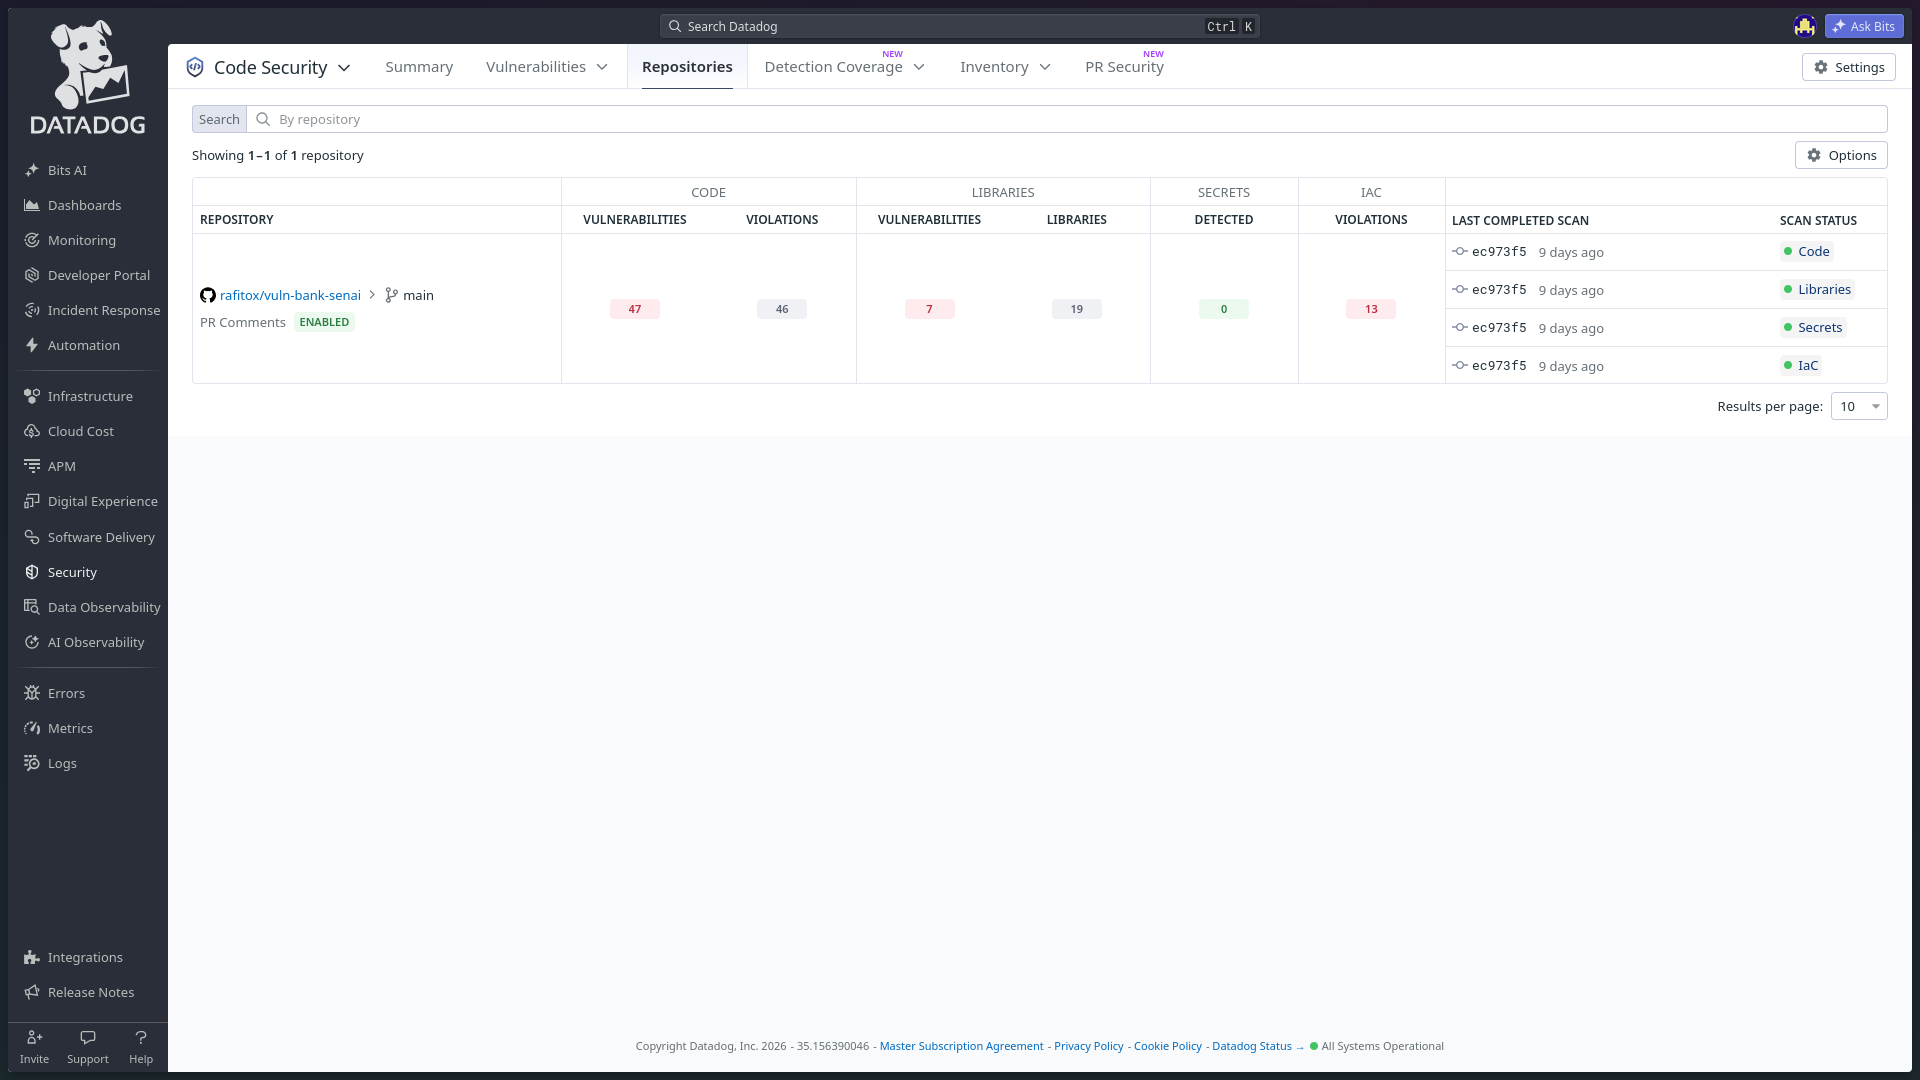
\includegraphics[width=0.88\textwidth]{assets/figures/datadog-repository.png}
\caption{Vista de repositórios na Datadog: o repositório
\texttt{rafitox/vuln-bank-senai} aparece com 47 vulnerabilidades
(46 violações), 7 vulnerabilidades de biblioteca em 19 bibliotecas, 0 segredos
detectados e 13 violações de IaC. A ausência de segredos detected corrobora
o resultado do Semgrep \texttt{p/secrets}, que não encontrou credenciais no
commit publicado.}
\label{fig:datadog-repo}
\end{figure}

% ================================================================
\section{Correções Aplicadas}\label{sec:correcoes}

Foram aplicadas \textbf{45 correções} (\texttt{F-01} a \texttt{F-45}), codificadas
em \textbf{10 commits} que alteraram \textbf{22 arquivos} com 4.908 inserções e
518 removições. A tabela seguinte apresenta as correções de maior impacto.

\begin{table}[H]
\centering
\caption{Correções de maior impacto, com CWE associado.}
\begin{tabularx}{\textwidth}{@{}lXll@{}}
\toprule
\textbf{ID} & \textbf{Correção} & \textbf{CWE} & \textbf{Severidade} \\
\midrule
F-01 & Parâmetros vinculados em todos os 66 pontos de SQL & CWE-89 & Crítica \\
F-05 & Segredo JWT externo obrigatório, $\geq$32 caracteres, \texttt{HS256} único & CWE-287 & Crítica \\
F-09 & IDOR corrigido em rotas de usuário e de comerciante & CWE-639 & Alta \\
F-13 & PAN e CVV removidos das respostas de pagamento & CWE-359 & Crítica \\
F-21 & Validação de tipo de arquivo no servidor (magic bytes) & CWE-434 & Alta \\
F-24 & CORS amplo removido; origem restrita & CWE-942 & Alta \\
F-28 & Cabeçalhos de segurança (CSP, HSTS, X-Content-Type-Options) & CWE-693 & Média \\
F-32 & Senha em \texttt{argon2}; segredo do admin por variável de ambiente & CWE-798 & Alta \\
F-37 & \texttt{X-Forwarded-For} aceito apenas de proxies confiáveis & CWE-441 & Alta \\
F-38 & PAN e CVV gerados por \texttt{secrets} & CWE-330 & Média \\
F-40 & Conexão fixada no IP validado (anti DNS rebinding) & CWE-367 & Crítica \\
F-41 & Importação remota restrita a HTTPS & CWE-319 & Média \\
F-42 & Leitura do corpo remoto limitada a blocos de 64 KB & CWE-400 & Média \\
F-43 & Nome de arquivo com prefixo imprevisível & CWE-330 & Alta \\
F-45 & Verificação de loopback por \texttt{ipaddress} & CWE-184 & Média \\
\bottomrule
\end{tabularx}
\end{table}

\subsection*{Exemplo de correção}

A vulnerabilidade de DNS rebinding (F-40) ilustra o padrão das correções. Na
versão original, o endereço era resolvido para validação, mas o nome de
domínio era entregue ao cliente HTTP, que o resolvia \emph{novamente} para
conectar. Um servidor DNS controlado pelo atacante poderia responder com um
endereço público na primeira consulta e um endereço interno na segunda,
fazendo com que o endereço validado não fosse o endereço efetivamente
conectado.

\begin{figure}[H]
\centering
\begin{minipage}[t]{0.48\textwidth}
\textbf{Antes (vulnerável)}
\begin{lstlisting}[basicstyle=\ttfamily\footnotesize,frame=single,breaklines=true]
resolved = socket.getaddrinfo(
    parsed.hostname, port,
    proto=socket.IPPROTO_TCP,
)
for ... sockaddr in resolved:
    if ip.is_private or ip.is_loopback:
        return erro

resp = requests.get(image_url, ...)
\end{lstlisting}
\end{minipage}
\hfill
\begin{minipage}[t]{0.48\textwidth}
\textbf{Depois (corrigido)}
\begin{lstlisting}[basicstyle=\ttfamily\footnotesize,frame=single,breaklines=true]
addresses = _resolve_public_addresses(
    parsed.hostname, port)
if addresses is None:
    return erro

resp = _pinned_fetch(
    image_url, parsed, addresses)
\end{lstlisting}
\end{minipage}
\caption{A validação continua occorrendo, mas a conexão passa a ser aberta
diretamente contra o endereço validado, mantendo o nome original para o SNI
TLS, a verificação do certificado e o cabeçalho \texttt{Host}.}
\label{fig:rebinding}
\end{figure}

% ================================================================
\section{Riscos Residuais}\label{sec:riscos}

As correções não eliminam todo o risco. Os itens abaixo permanecem
documentados de forma explícita, e sua correção exige decisão de projeto ou
infraestrutura, não apenas alteração de código.

\begin{table}[H]
\centering
\caption{Riscos residuais identificados após a remediação.}
\begin{tabularx}{\textwidth}{@{}lXll@{}}
\toprule
\textbf{ID} & \textbf{Risco residual} & \textbf{CWE} & \textbf{Situação} \\
\midrule
R-01 & Senhas e PINs de usuário gravados em texto claro no banco & CWE-256 & Requer migração \\
R-02 & JWT mantido em \texttt{localStorage} & CWE-922 & Requer cookies \texttt{HttpOnly} \\
R-03 & Ausência de tokens anti-CSRF & CWE-352 & Requer middleware \\
R-04 & Criptografia de senhas de comerciante em \emph{legacy} SHA-256 & CWE-916 & Migração em andamento \\
R-05 & Endpoint interno protegido apenas por loopback & CWE-284 & Depende da topologia de rede \\
R-06 & GraphQL: exceções do \emph{resolver} chegam ao cliente & CWE-209 & Aberto \\
R-07 & Proteção de força bruta ausente na rota de login & CWE-307 & Aberto \\
R-08 & Exposição de \texttt{debug\_info} em contexto de demonstração & CWE-215 & Delimitado \\
R-11 & Contadores de limite de taxa por processo (gunicorn) & CWE-400 & Exige armazenamento compartilhado \\
\bottomrule
\end{tabularx}
\end{table}

Dois pontos merecem destaque. O item \textbf{R-11} significa que, com quatro
trabalhadores do gunicorn, o limite efetivo de requisições é quatro vezes o
valor configurado --- a proteção existe, mas opera com folga maior que a
pretendida. O item \textbf{R-05} depende do \emph{proxy} que publica a
aplicação: se o serviço for exposto diretamente, a checagem de loopback deixa
de ser uma barreira suficiente.

% ================================================================
\section{Conclusão}

A auditoria da aplicação \textit{VulnBank} identificou \textbf{82 achados
estáticos}, dos quais \textbf{63} eram de severidade \textsc{ERROR}, além de
\textbf{37 advisories} em dependências e \textbf{26 comentários de segurança}
apontados pela revisão assistida por modelo de linguagem. Após a remediação,
o cenário converge para um estado defensável:

\begin{itemize}
  \item \textbf{82 $\rightarrow$ 4} achados Semgrep, com \textbf{zero} erros
  de severidade \textsc{ERROR};
  \item \textbf{66 $\rightarrow$ 0} pontos de injeção SQL;
  \item \textbf{37 $\rightarrow$ 0} advisories de dependências;
  \item \textbf{48 / 48} verificações de exploração e endurecimento
  rejeitadas ou aprovadas conforme o critério;
  \item \textbf{13 / 13} testes automatizados preservando a funcionalidade
  original.
\end{itemize}

O trabalho demonstra que a combinação de análise estática com verificação
exploratória é essencial: a varredura apontou para \textbf{66} pontos de
injeção SQL, mas a verificação exploratória foi o que revelou que a proteção
de SSRF aparentemente correta --- que validava o endereço resolvido --- ainda
permitia o redirecionamento por DNS rebinding. Da mesma forma, o Dockerfile
mantinha um pin de \texttt{gunicorn} divergente do \texttt{requirements.txt},
o que faria a imagem publicada em produção carregar uma versão vulnerável
enquanto a auditoria reportava o problema como resolvido.

Permanecem \textbf{11 riscos residuais} explicitamente documentados, dos quais
quatro exigem migração de dados ou mudança de arquitetura. A recomendação
principal é resolver \textbf{R-01} (criptografia de senhas em repouso) e
\textbf{R-11} (limite de taxa distribuído) antes de qualquer exposição real
da aplicação.

% ================================================================
\section{Mapeamento dos Critérios de Avaliação}

\begin{table}[H]
\centering
\caption{Onde cada critério de avaliação é atendido neste relatório.}
\begin{tabularx}{\textwidth}{@{}lXl@{}}
\toprule
\textbf{Critério} & \textbf{Onde é atendido} \\
\midrule
Metodologia e ferramental              & Seção \ref{sec:metodologia} \\
Resultados da análise estática          & Seção \ref{sec:estatica} \\
Comparativo antes e depois              & Seção \ref{sec:resultados} \\
Evidência visual dos resultados        & Figuras \ref{fig:metricas}, \ref{fig:datadog-xss} e \ref{fig:datadog-repo} \\
Correções aplicadas com CWE            & Seção \ref{sec:correcoes} \\
Riscos residuais assumidos             & Seção \ref{sec:riscos} \\
Reprodutibilidade dos resultados       & Apêndice \ref{app:reproducao} \\
Referências bibliográficas              & Seção \ref{sec:referencias} \\
\bottomrule
\end{tabularx}
\end{table}

\section{Referências Bibliográficas}\label{sec:referencias}

\begin{enumerate}[label={[\arabic*]}]
  \item OWASP Foundation. \textit{OWASP Top 10:2021 --- The ten most critical
  web application security risks}. 2021. Disponível em:
  \url{https://owasp.org/Top10/}. Acesso em: 24 nov. 2026.

  \item MITRE. \textit{Common Weakness Enumeration (CWE)}. MITRE Corporation.
  Disponível em: \url{https://cwe.mitre.org/}. Acesso em: 24 nov. 2026.

  \item OWASP Foundation. \textit{OWASP Testing Guide}. Version 4.0. 2020.
  Disponível em: \url{https://owasp.org/www-project-web-security-testing-guide/}.
  Acesso em: 24 nov. 2026.

  \item NIST. \textit{SP 800-115: Technical Guide to Information Security
  Testing and Assessment}. National Institute of Standards and Technology.
  \url{https://doi.org/10.6028/NIST.SP.800-115}.

  \item Semgrep. \textit{Semgrep --- Static Analysis for Security}. 2026.
  Disponível em: \url{https://semgrep.dev/}. Acesso em: 24 nov. 2026.

  \item Pypi Advisory Database. \textit{OSV --- Open Source Vulnerabilities}.
  2026. Disponível em: \url{https://osv.dev/}. Acesso em: 24 nov. 2026.

  \item Python Packaging Authority. \textit{pip-audit}. 2026. Disponível em:
  \url{https://pypi.org/project/pip-audit/}. Acesso em: 24 nov. 2026.

  \item Python Software Foundation. \textit{Python 3.12 Documentation:
  \texttt{secrets} --- Generate secure random numbers for managing secrets}.
  2026. \url{https://docs.python.org/3/library/secrets.html}.

  \item Python Software Foundation. \textit{PEP 493 --- Qualified name for
  Python packages}. 2015. \url{https://peps.python.org/pep-0493/}.

  \item IETF. \textit{RFC 7239 --- Forwarded HTTP Header}. 2014.
  \url{https://datatracker.ietf.org/doc/html/rfc7239}.

  \item IETF. \textit{RFC 6265 --- HTTP State Management Mechanism}. 2011.
  \url{https://datatracker.ietf.org/doc/html/rfc6265}.

  \item OWASP Foundation. \textit{OWASP Cheat Sheet Series: HTTP Headers
  Security}. 2026. \url{https://cheatsheetseries.owasp.org/cheatsheets/HTTP_Headers_Cheat_Sheet.html}.

  \item OWASP Foundation. \textit{OWASP Cheat Sheet Series: File Upload}.
  2026. \url{https://cheatsheetseries.owasp.org/cheatsheets/File_Upload_Cheat_Sheet.html}.

  \item OWASP Foundation. \textit{OWASP Cheat Sheet Sheet: SQL Injection
  Prevention}. 2026. \url{https://cheatsheetseries.owasp.org/cheatsheets/SQL_Injection_Prevention_Cheat_Sheet.html}.

  \item OWASP Foundation. \textit{OWASP Cheat Sheet Series: Server Side
  Request Forgery Prevention}. 2026.
  \url{https://cheatsheetseries.owasp.org/cheatsheets/Server_Side_Request_Forgery_Prevention_Cheat_Sheet.html}.

  \item PCI Security Standards Council. \textit{PCI DSS v4.0 --- Payment Card
  Industry Data Security Standard}. 2024.
  \url{https://www.pcisecuritystandards.org/standards/pci-dss/}.

  \item cloudflare. \textit{Cloudflare WAF and DDoS Protection}. 2026.
  Disponível em: \url{https://developers.cloudflare.com/waf/}. Acesso em:
  24 nov. 2026.

  \item Datadog. \textit{Code Security --- Application Security Testing}.
  2026. \url{https://docs.datadoghq.com/code_security/}. Acesso em:
  24 nov. 2026.

  \item Martin, R. C. \textit{Clean Code: A Handbook of Agile Software
  Craftsmanship}. Prentice Hall, 2008.

  \item McConnell, S. \textit{Code Complete: A Comprehensive Handbook of
  Software Construction}. 2nd ed. Addison-Wesley, 2004.
\end{enumerate}

\appendix
\section{Reprodução}
\label{app:reproducao}

\subsection{Repositório e branch}

\begin{verbatim}
git clone git@github.com:rafitox/vuln-bank-SENAI.git
cd vuln-bank
git checkout security/remediation-2026-11
\end{verbatim}

O commit \texttt{main} (\texttt{ec973f5}) foi preservado sem alteração, porque
o workflow \texttt{deploy.yml} executa um deploy real a cada push nessa
branch. Todo o trabalho está isolado na branch de remediação.

\subsection{Validação do estado final}

\begin{verbatim}
# Testes automatizados
python -m pytest tests/ -q

# Suítes de verificação de segurança
python .audit/verify_exploits.py     # 13/13
python .audit/verify_uploads.py      # 14/14
python .audit/test_ssrf.py           # 8/8
python .audit/test_rebind.py         # DNS rebinding
python .audit/test_hardening.py      # 21/21

# Análise estática
semgrep scan --config p/default --config p/security-audit \
  --config p/flask --config p/python --config p/secrets
\end{verbatim}

\subsection{Commits de remediação}

\begin{verbatim}
79db613  fix(security): remediate SAST and audit findings
b2af587  fix(upload): validate profile picture type and size
2be7d11  docs: add visual before/after comparison page
15ed202  fix(security): address findings from the post-remediation OCR review
33ec82b  docs: refresh comparison page with the eight new findings
6fedc78  fix(ssrf): pin the outbound connection to the validated address
9a492af  refactor(ssrf): remove the duplicated address resolver
3ba3871  fix(security): bound the remote read and remove weak randomness
5e70288  docs: refresh comparison page with SSRF and rate-limit findings
e3c2556  docs: refresh comparison page with bounded-read findings
\end{verbatim}

\end{document}
